\section{Análisis distribucional}
\label{sec:analisis_distribucional}

% Distribuciones de cada feature con estadísticos descriptivos
% (media, mediana, IQR, outliers).
%
% Para cada feature: histograma o boxplot, media, mediana, desviación
% estándar, percentiles 5 y 95. Identificar features con distribución
% degenerada (e.g. masa puntual, valores constantes por trial).
%
% Analizar por separado features estáticas vs. dinámicas y, dentro
% de las dinámicas, la evolución a lo largo del trial (posición de
% fijación 1, 2, ..., k).
%
% Señalar features candidatas a transformación (log, normalización)
% antes del modelado.

Se presenta el análisis distribucional de las features.

El análisis se organiza en torno a dos perspectivas complementarias:
\begin{itemize}
    \item \textbf{Análisis global:} se presentan histogramas y estadísticos descriptivos para cada feature, considerando el conjunto completo de fijaciones del dataset ($N = 61.252$). Esto permite identificar características generales de la distribución, como sesgo, presencia de outliers o valores constantes.
    
    \item \textbf{Mirada por sujeto:} se examina la variabilidad de cada feature dentro de cada participante por separado. El modelo de regresión \todo{ver como nombrar modelo} se estima de forma independiente para cada sujeto: la matriz de diseño de cada participante contiene únicamente sus propias fijaciones, y los coeficientes TRF resultantes reflejan la relación entre las features y la señal cerebral de ese individuo. En consecuencia, es crucial verificar que las features presentan variabilidad dentro de cada sujeto, ya que una feature constante para un participante no contribuirá a explicar su señal cerebral.
\end{itemize}


\subsection{Análisis Global}
\subsubsection{Información Bottom Up}

Las features de información bottom-up se encuentran sesgadas a la derecha, con una mayoría de fijaciones que presentan valores bajos. Esto refleja que la mayoría de las fijaciones caen en zonas de baja saliencia. 

\begin{table}[H]
\centering
\caption{Estadísticos descriptivos de las features de información bottom-up.}
\label{tab:dist_bottomup}
\small
\setlength{\tabcolsep}{8pt}
\renewcommand{\arraystretch}{1.2}
\begin{tabular}{lrrr}
\toprule
 & \texttt{saliencia\_media} & \texttt{saliencia\_mediana} & \texttt{saliencia\_pixel} \\
\midrule
count & 61252 & 61252 & 61252 \\
mean  & 0.1046 & 0.1004 & 0.0449 \\
std   & 0.1408 & 0.1391 & 0.0954 \\
min   & 0.0000 & 0.0000 & 0.0000 \\
25\%  & 0.0164 & 0.0157 & 0.0000 \\
50\%  & 0.0507 & 0.0471 & 0.0078 \\
75\%  & 0.1309 & 0.1255 & 0.0431 \\
max   & 0.9010 & 0.9059 & 1.0000 \\
\bottomrule
\end{tabular}
\end{table}

\subsubsection{Similitud con el target}

Al igual que las features de información bottom-up, las features de información similitud con el target también se encuentran sesgadas a la derecha, con una mayoría de fijaciones con valores bajos.

\begin{table}[H]
\centering
\caption{Estadísticos descriptivos de las features de similitud con el target.}
\label{tab:dist_similitud}
\small
\setlength{\tabcolsep}{8pt}
\renewcommand{\arraystretch}{1.2}
\begin{tabular}{lrrr}
\toprule
 & \texttt{similitud\_media} & \texttt{similitud\_mediana} & \texttt{similitud\_pixel} \\
\midrule
count & 61252 & 61252 & 61252 \\
mean  & 0.0910 & 0.0835 & 0.0334 \\
std   & 0.1172 & 0.1157 & 0.0715 \\
min   & 0.0000 & 0.0000 & 0.0000 \\
25\%  & 0.0133 & 0.0118 & 0.0039 \\
50\%  & 0.0452 & 0.0373 & 0.0078 \\
75\%  & 0.1251 & 0.1098 & 0.0314 \\
max   & 0.8268 & 0.8353 & 0.9490 \\
\bottomrule
\end{tabular}
\end{table}

\subsubsection{Estado interno del proceso bayesiano}

\todo{Pendiente: análisis de las features de competencia fp}

La feature \texttt{posterior} es la que presenta mayor sesgo de todo el conjunto. Su distribución se encuentra extremadamente concentrada cerca de cero, con una cola muy larga hacia valores altos. Esto es esperable dado el funcionamiento del modelo bayesiano nnELM: en cada fijación, la probabilidad asignada a la celda fijada es muy pequeña, salvo en las fijaciones finales cuando la posterior se concentra en torno al target. La concentración de \texttt{posterior} hacia el final del trial se analiza en la sección~\ref{sec:coherencia_busqueda}.

\begin{table}[H]
\centering
\caption{Estadísticos descriptivos de las features dinámicas del estado interno (parte I).}
\label{tab:dist_bayesiano_a}
\small
\setlength{\tabcolsep}{4pt}
\renewcommand{\arraystretch}{1.2}
\resizebox{\linewidth}{!}{%
\begin{tabular}{lrrrrr}
\toprule
 & \texttt{evidencia\_visual} & \texttt{competencia\_fp\_var} & \texttt{competencia\_fp\_media} & \texttt{competencia\_fp\_max} & \texttt{posterior} \\
\midrule
count & 61252    & 61252   & 61252    & 61252         & 61252        \\
mean  & $-3.36$  & 4.60    & $-0.195$ & 4.83          & 0.0152       \\
std   & 2.28     & 1.58    & 0.0835   & 10.3          & 0.0939       \\
min   & $-8.91$  & 0.231   & $-0.342$ & ${\approx}0$  & ${\approx}0$ \\
25\%  & $-4.69$  & 3.50    & $-0.243$ & 0.0307        & 0.00000506   \\
50\%  & $-3.76$  & 4.50    & $-0.217$ & 0.484         & 0.0000230    \\
75\%  & $-2.71$  & 5.59    & $-0.183$ & 3.53          & 0.0000980    \\
max   & 8.44     & 13.6    & 0.298    & 74.2          & 1.00         \\
\bottomrule
\end{tabular}%
}
\end{table}

La distribución de \texttt{entropia\_prior\_saliencia} es estrecha (std $= 0.447$), lo que indica que las imágenes del dataset presentan una complejidad visual similar entre sí. El valor máximo para una distribución uniforme sobre la grilla de $24 \times 32 = 768$ celdas es $\log(768) \approx 6.64$; dado que la media se ubica en $5.45$, los mapas de saliencia presentan siempre cierta estructura espacial, sin ser completamente uniformes ni extremadamente concentrados.

Por otro lado, la mediana de \texttt{entropia\_posterior} se ubica en $6.10$, lo que indica una posterior casi uniforme sobre la grilla en la mayoría de las fijaciones. La evolución de esta feature a lo largo del trial se examina en la sección~\ref{sec:coherencia_busqueda}.

La distribución de \texttt{ganancia\_informacion} está fuertemente sesgada a la derecha (mediana $= 0.052$, media $= 0.214$, máximo $= 5.90$), lo que indica que la mayoría de las fijaciones aportan poca información sobre la localización del target. Se analiza si las fijaciones con ganancia alta se concentran hacia el final del trial en la sección~\ref{sec:coherencia_busqueda}.

\begin{table}[H]
\centering
\caption{Estadísticos descriptivos de las features del estado interno (parte II): entropías y ganancia.}
\label{tab:dist_bayesiano_b}
\small
\setlength{\tabcolsep}{8pt}
\renewcommand{\arraystretch}{1.2}
\begin{tabular}{lrrr}
\toprule
 & \texttt{entropia\_prior\_saliencia} & \texttt{entropia\_posterior} & \texttt{ganancia\_informacion} \\
\midrule
count & 61252 & 61252   & 56751   \\
mean  & 5.45  & 5.35    & 0.214   \\
std   & 0.447 & 1.71    & 0.456   \\
min   & 3.85  & 0.0000140 & 0.00000300 \\
25\%  & 5.28  & 5.37    & 0.0257  \\
50\%  & 5.48  & 6.10    & 0.0517  \\
75\%  & 5.79  & 6.38    & 0.143   \\
max   & 6.15  & 6.58    & 5.90    \\
\bottomrule
\end{tabular}
\end{table}

\subsubsection{Calidad de la decisión}

La feature \texttt{gap\_entropia} cuantifica la diferencia entre la ganancia
de información esperada en la fijación óptima según el modelo y la ganancia
correspondiente a la fijación efectivamente realizada por el sujeto. Su
distribución presenta un marcado sesgo a la derecha: la mediana es $0.262$
pero la media asciende a $0.711$, con un máximo de $4.48$, lo que indica
que la mayoría de las fijaciones se alejan moderadamente del óptimo pero
existen casos de suboptimalidad muy pronunciada. El mínimo exactamente igual
a $0$ refleja los casos en que el sujeto fija la celda óptima según el
criterio ELM. En conjunto, la distribución revela una suboptimalidad
sistemática: los sujetos no siguen la estrategia de minimización de
entropía que prescribe el modelo. \todo{esto es esperable? Buscar y citar}

Las features \texttt{distancia\_grilla} (mediana $= 9.43$ celdas) y
\texttt{distancia\_pixels} (mediana $= 302$ px) complementan este análisis
desde una perspectiva espacial. Dado que la grilla tiene $32$ columnas,
una distancia mediana de $9.43$ celdas equivale casi a un tercio del ancho
de la imagen, indicando que la mayoría de las fijaciones se encuentran
a una distancia considerable del óptimo, coherente con el análisis de
\texttt{gap\_entropia}.

\begin{table}[H]
\centering
\caption{Estadísticos descriptivos de las features de calidad de la decisión.}
\label{tab:dist_decision}
\small
\setlength{\tabcolsep}{8pt}
\renewcommand{\arraystretch}{1.2}
\begin{tabular}{lrrr}
\toprule
 & \texttt{gap\_entropia} & \texttt{distancia\_grilla} & \texttt{distancia\_pixels} \\
\midrule
count & 56751  & 56751  & 56751  \\
mean  & 0.711  & 9.91   & 317    \\
std   & 1.04   & 6.03   & 193    \\
min   & 0.000  & 0.000  & 0.000  \\
25\%  & 0.127  & 5.39   & 172    \\
50\%  & 0.262  & 9.43   & 302    \\
75\%  & 0.702  & 13.9   & 446    \\
max   & 4.48   & 31.8   & 1016   \\
\bottomrule
\end{tabular}
\end{table}

\subsubsection{Competencia entre candidatos}

La feature \texttt{competencia\_ratio} presenta una baja variabilidad relativa (std $= 0.056$, media $= 0.927$), lo que indica que casi siempre el segundo mejor candidato alcanza entre el $89\%$ y el $97\%$ del valor del mejor candidato. En otras palabras, el mapa EIG rara vez tiene un único ganador claro: casi siempre hay competencia entre candidatos.

\begin{table}[H]
\centering
\caption{Estadísticos descriptivos de las features de competencia entre candidatos.}
\label{tab:dist_competencia}
\small
\setlength{\tabcolsep}{7pt}
\renewcommand{\arraystretch}{1.2}
\begin{tabular}{lrrr}
\toprule
 & \texttt{competencia\_ratio} & \texttt{competencia\_densidad} & \texttt{competencia\_densidad\_norm} \\
\midrule
count & 61252  & 61252  & 61252   \\
mean  & 0.927  & 1.79   & 0.00233 \\
std   & 0.0562 & 1.82   & 0.00237 \\
min   & 0.763  & 1.00   & 0.00130 \\
25\%  & 0.889  & 1.00   & 0.00130 \\
50\%  & 0.940  & 1.00   & 0.00130 \\
75\%  & 0.974  & 2.00   & 0.00260 \\
max   & 1.00   & 96.0   & 0.125   \\
\bottomrule
\end{tabular}
\end{table}

\subsubsection{Análisis General}

La Figura~\ref{fig:violin_plot_features} presenta la distribución de las 
22 features estandarizadas (z-score) mediante violinplots, agrupadas por 
categoría. La estandarización permite comparar la forma y dispersión 
relativa de todas las features en un mismo eje, independientemente de 
sus unidades y escalas originales. Las líneas internas de cada violín 
indican la mediana y los cuartiles Q1 y Q3 de la distribución.

\begin{figure}[H]
    \centering
    \makebox[\textwidth][c]{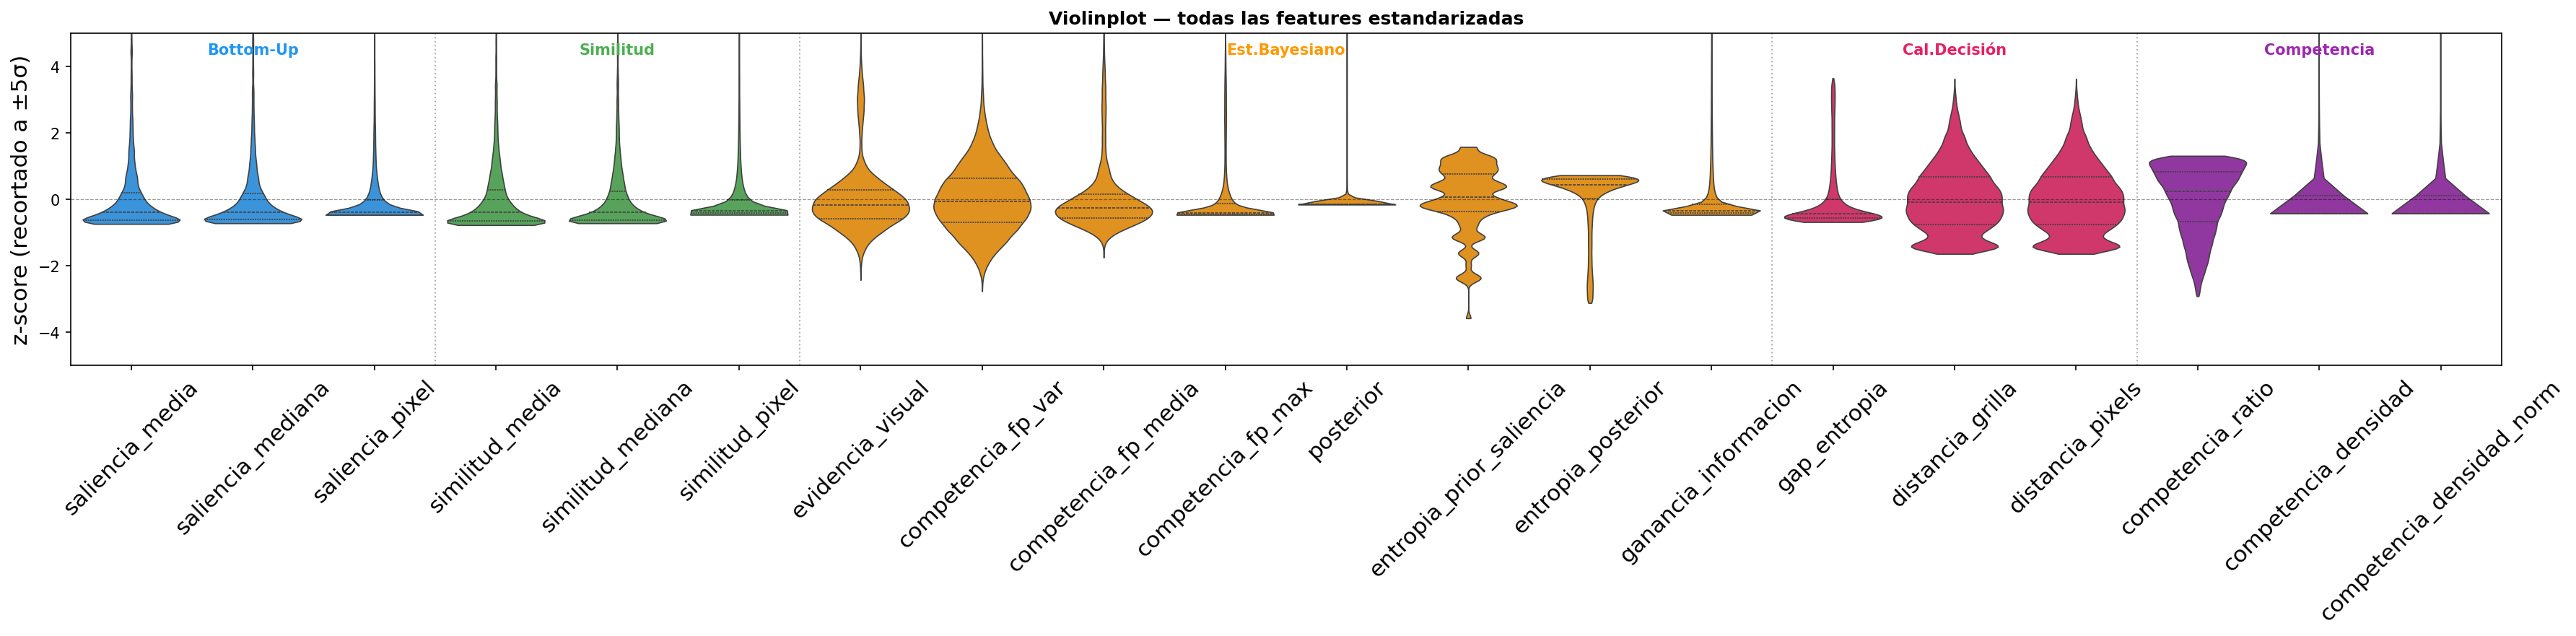
\includegraphics[width=1.3\textwidth]{chapters/03_analisis_features/images/violin_plot_features}}
    \caption{Distribución de las features extraídas del modelo nnELM. Cada violín muestra la densidad empírica de la feature correspondiente sobre el conjunto completo de fijaciones ($N = 61.252$).}
    \label{fig:violin_plot_features}
\end{figure}


El análisis de los violinplots permite identificar patrones 
distribucionales relevantes que complementan los estadísticos 
descriptivos de las tablas anteriores. Se observan las diferencias en la forma de las 
distribuciones. Las features \texttt{evidencia\_visual} y 
\texttt{competencia\_fp\_media} son las únicas con distribuciones 
aproximadamente simétricas. El resto presenta asimetría en alguna 
dirección: las features \texttt{posterior}, \texttt{ganancia\_informacion}, 
\texttt{competencia\_fp\_max}, \texttt{gap\_entropia} y 
\texttt{competencia\_densidad} muestran una cola pronunciada hacia 
valores positivos, con masa concentrada en valores bajos y eventos 
raros de valores altos. En sentido contrario, \texttt{entropia\_posterior} 
y \texttt{competencia\_ratio} presentan una cola hacia valores negativos, 
con la masa concentrada en la parte alta de su rango.

\subsection{Mirada por sujeto}

La variabilidad relevante para el modelo de TRFs por regresión regularizada no es la variabilidad global del dataset sino la variabilidad dentro de cada sujeto (variabilidad within-subject). El objetivo de esta sección es analizar cuánto varía cada feature dentro de las fijaciones de un mismo participante. Para cuantificarla se calcularon las siguientes métricas, tomando como unidad de análisis a cada sujeto por separado:

\todo{Esto esta ok acá o debería ir en métodos?}

Para cada sujeto $s$ y cada feature $f$, se calculó el desvío estándar de los valores de $f$ sobre todas sus fijaciones:

\begin{equation}
    \sigma_{f,s} = \text{std}\left(\{f_t : t \in \text{fijaciones de } s\}\right)
\end{equation}

A partir de este valor se derivaron dos métricas de resumen:

\begin{itemize}
    \item \textbf{Std within-subject mediano} ($\widetilde{\sigma}_f$): 
    mediana de $\sigma_{f,s}$ entre los $S = 44$ sujetos. Cuantifica 
    cuánto varía típicamente la feature dentro de un participante, en 
    las unidades originales de la feature.

    \item \textbf{Coeficiente de variación within-subject mediano} 
    ($\widetilde{CV}_f$): mediana del cociente $\frac{\sigma_{f,s} }{\mu_{f,s}}$
    donde $\mu_{f,s}$ es la media de la feature para el sujeto $s$. Al 
    normalizar por la media, esta métrica es adimensional y permite 
    comparar features en distintas escalas. Un valor de $\widetilde{CV}_f = 0.1$ 
    indica que el desvío estándar within-subject es el $10\%$ de la media.

\end{itemize}

La Tabla~\ref{tab:within_subject} presenta las tres métricas calculadas
para cada feature, ordenadas de menor a mayor coeficiente de variación
within-subject.

\begin{table}[H]
\centering
\caption{Variabilidad within-subject de cada feature}
\label{tab:within_subject}
\small
\setlength{\tabcolsep}{8pt}
\renewcommand{\arraystretch}{1.2}
\begin{tabular}{lrrl}
\toprule
\textbf{Feature} & $\widetilde{\sigma}_f$ & $\widetilde{CV}_f$ & \textbf{Categoría} \\
\midrule
\texttt{competencia\_ratio}           & 0.0558  & 0.060 & Competencia       \\
\texttt{entropia\_prior\_saliencia}   & 0.4461  & 0.082 & Est.\ Bayesiano   \\
\texttt{entropia\_posterior}          & 1.6322  & 0.304 & Est.\ Bayesiano   \\
\texttt{competencia\_fp\_var}         & 1.5731  & 0.342 & Est.\ Bayesiano   \\
\texttt{competencia\_fp\_media}       & 0.0811  & 0.416 & Est.\ Bayesiano   \\
\texttt{distancia\_pixels}            & 191.399 & 0.603 & Cal.\ Decisión    \\
\texttt{distancia\_grilla}            & 5.9812  & 0.603 & Cal.\ Decisión    \\
\texttt{evidencia\_visual}            & 2.2432  & 0.647 & Est.\ Bayesiano   \\
\texttt{competencia\_densidad}        & 1.4914  & 0.822 & Competencia       \\
\texttt{competencia\_densidad\_norm}  & 0.0019  & 0.822 & Competencia       \\
\texttt{similitud\_media}             & 0.1150  & 1.278 & Similitud         \\
\texttt{saliencia\_media}             & 0.1416  & 1.333 & Bottom-Up         \\
\texttt{similitud\_mediana}           & 0.1137  & 1.369 & Similitud         \\
\texttt{saliencia\_mediana}           & 0.1397  & 1.372 & Bottom-Up         \\
\texttt{gap\_entropia}                & 1.0026  & 1.469 & Cal.\ Decisión    \\
\texttt{ganancia\_informacion}        & 0.4512  & 2.111 & Est.\ Bayesiano   \\
\texttt{saliencia\_pixel}             & 0.0959  & 2.123 & Bottom-Up         \\
\texttt{competencia\_fp\_max}         & 9.9494  & 2.132 & Est.\ Bayesiano   \\
\texttt{similitud\_pixel}             & 0.0718  & 2.133 & Similitud         \\
\texttt{posterior}                    & 0.0874  & 6.468 & Est.\ Bayesiano   \\
\bottomrule
\end{tabular}
\end{table}

La feature \texttt{competencia\_ratio} presenta el coeficiente de variación within-subject más bajo del conjunto ($\widetilde{CV} = 0.060$), consistente
con su distribución global estrecha ya observada en el análisis distribucional
(std $= 0.056$, rango $[0.763,\, 1.000]$). Dado que esta feature es casi
constante tanto a nivel global como dentro de cada sujeto, se la considera
candidata a descarte antes del modelado de EEG. \todo{Chequear si tiene sentido con los resultados en el modelo de TRFs. Ver si agregar esos resultados o ya la damos x descartada}

La feature \texttt{entropia\_prior\_saliencia} también presenta un
$\widetilde{CV}$ bajo ($0.082$), pero es esperable al ser
estática por trial. Su variabilidad within-subject no refleja la dinámica 
de búsqueda fijación a fijación sino únicamente las diferencias entre las 
imágenes vistas por cada participante. Esta característica no implica 
degeneración, y es consistente con lo observado en el análisis distribucional: 
la estrechez de su distribución global (std $= 0.447$, rango $[3.85,\, 6.15]$ 
frente al máximo teórico de $\ln(768) \approx 6.64$ nats) refleja que las 
imágenes del dataset presentan una complejidad visual similar entre sí, 
lo que naturalmente limita la variabilidad de esta feature tanto entre 
trials como dentro de cada sujeto.

En el extremo opuesto, las features de saliencia y similitud presentan 
coeficientes de variación superiores a $1$, lo que indica que su desvío 
estándar within-subject supera a su propia media. Lo mismo ocurre con 
\texttt{ganancia\_informacion} ($\widetilde{CV} = 2.111$), 
\texttt{competencia\_fp\_max} ($\widetilde{CV} = 2.132$) y 
\texttt{similitud\_pixel} ($\widetilde{CV} = 2.133$). Estas features 
presentan la mayor variabilidad relativa dentro de cada sujeto y son 
por lo tanto las candidatas más robustas como predictores individuales.

Es importante considerar una limitación del coeficiente de variación como 
métrica de variabilidad: al ser un cociente entre el desvío estándar y la 
media, su valor se infla artificialmente cuando la media es cercana a cero 
pero el desvío estándar no lo es proporcionalmente. En ese caso, un CV 
alto no refleja necesariamente una feature con gran variabilidad 
within-subject sino simplemente una feature cuya media es pequeña en 
relación a su dispersión.

Esta situación se presenta en \texttt{posterior} ($\mu = 0.0135$, 
$\widetilde{\sigma} = 0.087$), \texttt{similitud\_pixel} ($\mu = 0.0337$, 
$\widetilde{\sigma} = 0.072$) y \texttt{saliencia\_pixel} ($\mu = 0.0450$, 
$\widetilde{\sigma} = 0.096$): las tres tienen medias pequeñas pero 
desvíos estándar considerablemente mayores que sus medias, lo que infla 
el cociente. Esto contrasta con \texttt{competencia\_densidad\_norm}, 
que también tiene media pequeña ($\mu = 0.00231$) pero cuyos valores 
están igualmente agrupados cerca de cero ($\widetilde{\sigma} = 0.0019$), 
resultando en un CV moderado ($0.822$). Por esta razón, el CV de las 
tres features mencionadas debe interpretarse con cuidado y complementarse 
con el análisis de su distribución global presentado en la sección 
anterior.